\documentclass[conference]{IEEEtran}
\IEEEoverridecommandlockouts
% The preceding line is only needed to identify funding in the first footnote. If that is unneeded, please comment it out.
\usepackage{cite}
\usepackage{amsmath,amssymb,amsfonts}
\usepackage{algorithmic}
\usepackage{graphicx}
\usepackage{textcomp}
\usepackage{xcolor}
\usepackage{listings}                           %顯示code用的
\usepackage{fontspec}                           %設定字體
\usepackage[CheckSingle, CJKmath]{xeCJK}
\usepackage{CJKulem}
\usepackage{listings}
\usepackage{color} %red, green, blue, yellow, cyan, magenta, black, white
\usepackage{float}

\definecolor{mygreen}{RGB}{28,172,0} % color values Red, Green, Blue
\definecolor{mylilas}{RGB}{170,55,241}

\setmainfont{Consolas}
%\setmonofont{Ubuntu Mono}
\setmonofont{Consolas}
\setCJKmainfont{Noto Sans CJK TC}
\XeTeXlinebreaklocale "zh"                      %中文自動換行

\lstset{language=Matlab,%
    %basicstyle=\color{red},
    breaklines=true,%
    morekeywords={matlab2tikz},
    keywordstyle=\color{blue},%
    morekeywords=[2]{1}, keywordstyle=[2]{\color{black}},
    identifierstyle=\color{black},%
    stringstyle=\color{mylilas},
    commentstyle=\color{mygreen},%
    showstringspaces=false,%without this there will be a symbol in the places where there is a space
    numbers=left,%
    numberstyle={\tiny \color{black}},% size of the numbers
    numbersep=9pt, % this defines how far the numbers are from the text
    emph=[1]{for,end,break},emphstyle=[1]\color{red}, %some words to emphasise
    %emph=[2]{word1,word2}, emphstyle=[2]{style},    
}

\def\BibTeX{{\rm B\kern-.05em{\sc i\kern-.025em b}\kern-.08em
    T\kern-.1667em\lower.7ex\hbox{E}\kern-.125emX}}

\begin{document}
\title{Digital Image Processing-Assignment 02\\
% {\footnotesize \textsuperscript{*}Note: Sub-titles are not captured in Xplore and should not be used}
% \thanks{Identify applicable funding agency here. If none, delete this.}
}

\author{\IEEEauthorblockN{1\textsuperscript{st} Zih Jie Lin}
\IEEEauthorblockA{\textit{Computer Science Information Engineering.} \\
\textit{Fu Jen Catholoic University}\\
New Taipei City, Taiwan \\
406261597@gapp.fju.edu.tw}
}
% \and
% \IEEEauthorblockN{2\textsuperscript{nd} Given Name Surname}
% \IEEEauthorblockA{\textit{dept. name of organization (of Aff.)} \\
% \textit{name of organization (of Aff.)}\\
% City, Country \\
% email address or ORCID}
% \and
% \IEEEauthorblockN{3\textsuperscript{rd} Given Name Surname}
% \IEEEauthorblockA{\textit{dept. name of organization (of Aff.)} \\
% \textit{name of organization (of Aff.)}\\
% City, Country \\
% email address or ORCID}
% \and
% \IEEEauthorblockN{4\textsuperscript{th} Given Name Surname}
% \IEEEauthorblockA{\textit{dept. name of organization (of Aff.)} \\
% \textit{name of organization (of Aff.)}\\
% City, Country \\
% email address or ORCID}
% \and
% \IEEEauthorblockN{5\textsuperscript{th} Given Name Surname}
% \IEEEauthorblockA{\textit{dept. name of organization (of Aff.)} \\
% \textit{name of organization (of Aff.)}\\
% City, Country \\
% email address or ORCID}
% \and
% \IEEEauthorblockN{6\textsuperscript{th} Given Name Surname}
% \IEEEauthorblockA{\textit{dept. name of organization (of Aff.)} \\
% \textit{name of organization (of Aff.)}\\
% City, Country \\
% email address or ORCID}

\maketitle

% \begin{abstract}
% \end{abstract}

% \begin{IEEEkeywords}
% \end{IEEEkeywords}

\section{實驗說明}
調整 window size, $\sigma$, threshold 參數,觀察是否有改變。

\begin{itemize}
\item window size: $3,5,7$
\item $\sigma$: $0.1,0.3,0.5,0.7,0.9$
\item threshold: $0,10,20,30,40,50$
\item 圖片: lena, headCT 
\end{itemize}

\section{程式碼}
\lstinputlisting{problem.m}

\section{成果}
\subsection{Lena}

原圖

\begin{figure}[H]
\centerline{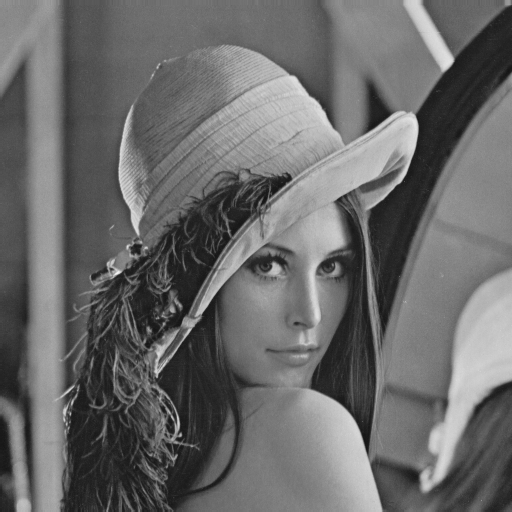
\includegraphics[width=8cm]{lena.png}}
\caption{lena}
\label{lena}
\end{figure}

不同的 window size: window size 越大,黑色部分就會越粗。

\begin{figure}[H]
\centerline{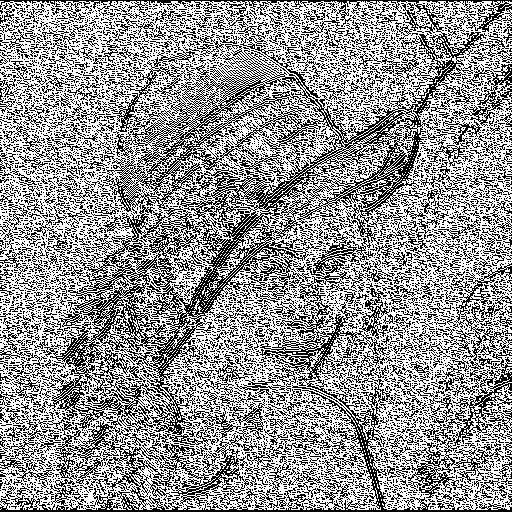
\includegraphics[width=8cm]{lena01.png}}
\caption{window size = $3$, $\sigma=0.3$,  threshold = $30$}
\label{lena01}
\end{figure}

\begin{figure}[H]
\centerline{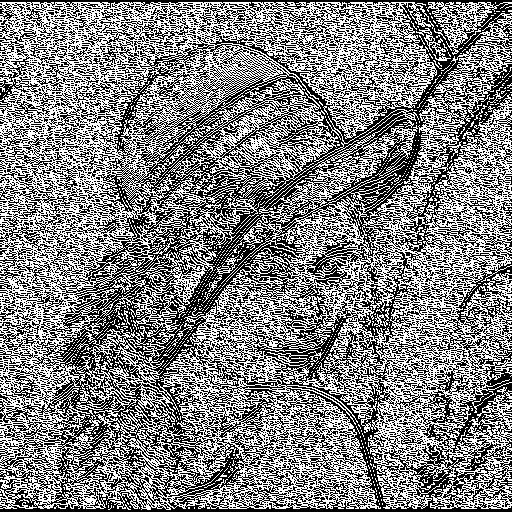
\includegraphics[width=8cm]{lena02.png}}
\caption{window size = $5$, $\sigma=0.3$,  threshold = $30$}
\label{lena02}
\end{figure}

\begin{figure}[H]
\centerline{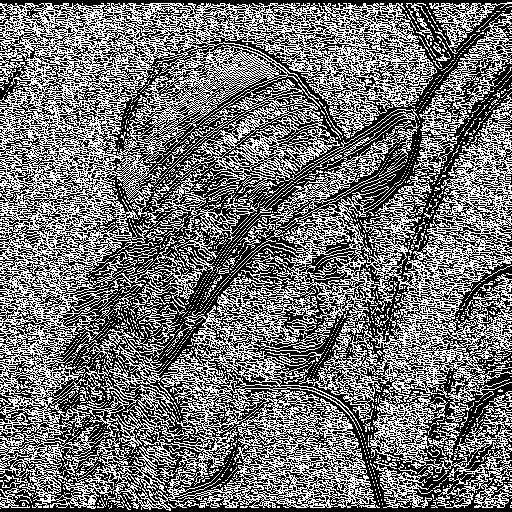
\includegraphics[width=8cm]{lena03.png}}
\caption{window size = $7$, $\sigma=0.3$,  threshold = $30$}
\label{lena03}
\end{figure}

不同的 $\sigma$:$\sigma$ 越大,黑白的區隔越明顯。


\begin{figure}[H]
\centerline{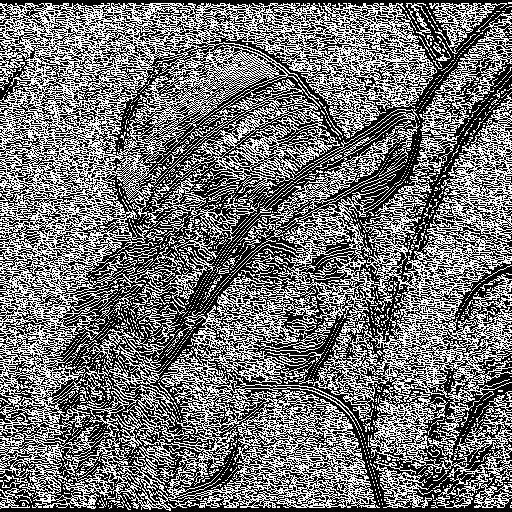
\includegraphics[width=8cm]{lena04.png}}
\caption{window size = $7$, $\sigma=0.1$,  threshold = $40$}
\label{lena04}
\end{figure}

\begin{figure}[H]
\centerline{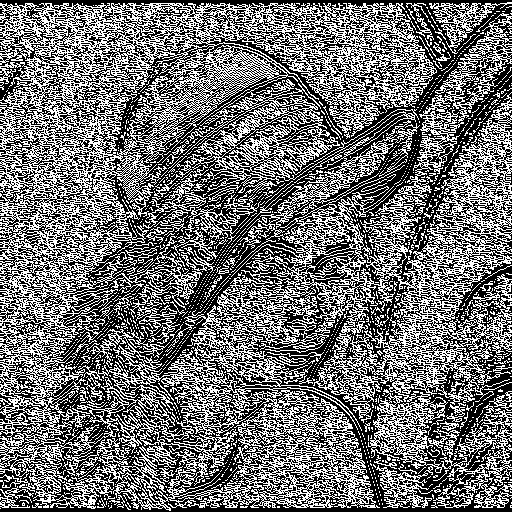
\includegraphics[width=8cm]{lena05.png}}
\caption{window size = $7$, $\sigma=0.3$,  threshold = $40$}
\label{lena05}
\end{figure}

\begin{figure}[H]
\centerline{
\includegraphics[width=8cm]{lena06.png}}
\caption{window size = $7$, $\sigma=0.5$,  threshold = $40$}
\label{lena06}
\end{figure}

\begin{figure}[H]
\centerline{
\includegraphics[width=8cm]{lena07.png}}
\caption{window size = $7$, $\sigma=0.7$,  threshold = $40$}
\label{lena07}
\end{figure}

\begin{figure}[H]
\centerline{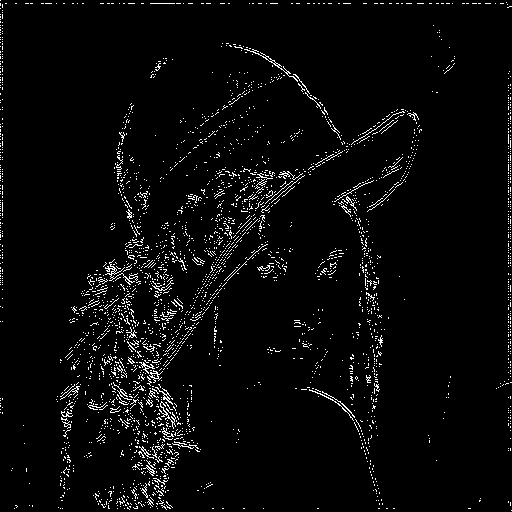
\includegraphics[width=8cm]{lena08.png}}
\caption{window size = $7$, $\sigma=0.9$,  threshold = $40$}
\label{lena08}
\end{figure}

不同的 thresold: thresold 越大,白色的區域減少。

\begin{figure}[H]
\centerline{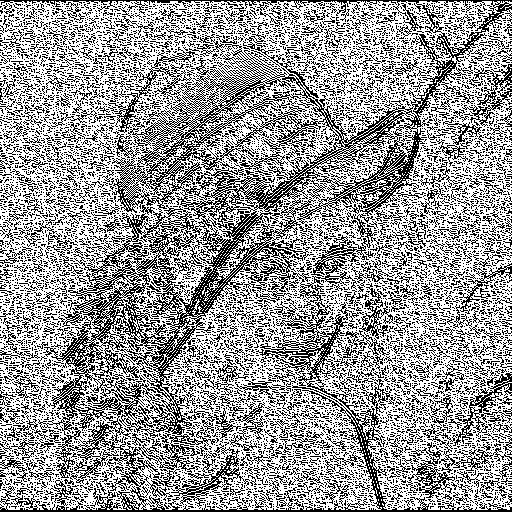
\includegraphics[width=8cm]{lena09.png}}
\caption{window size = $3$, $\sigma=0.5$,  threshold = $0$}
\label{lena9}
\end{figure}

\begin{figure}[H]
\centerline{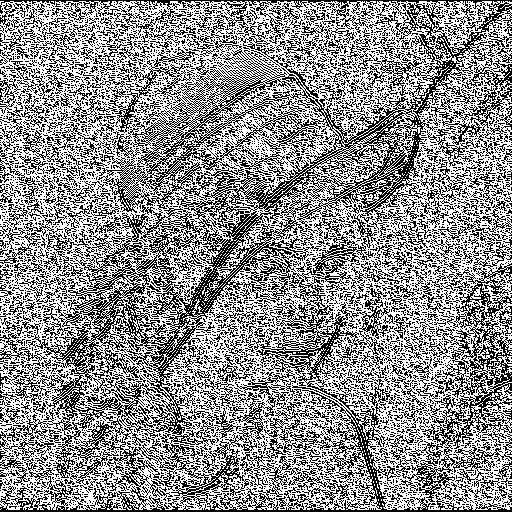
\includegraphics[width=8cm]{lena10.png}}
\caption{window size = $3$, $\sigma=0.5$,  threshold = $10$}
\label{lena10}
\end{figure}

\begin{figure}[H]
\centerline{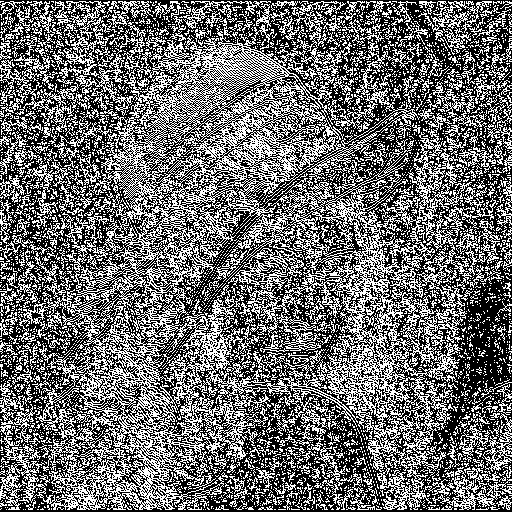
\includegraphics[width=8cm]{lena11.png}}
\caption{window size = $3$, $\sigma=0.5$,  threshold = $20$}
\label{lena11}
\end{figure}

\begin{figure}[H]
\centerline{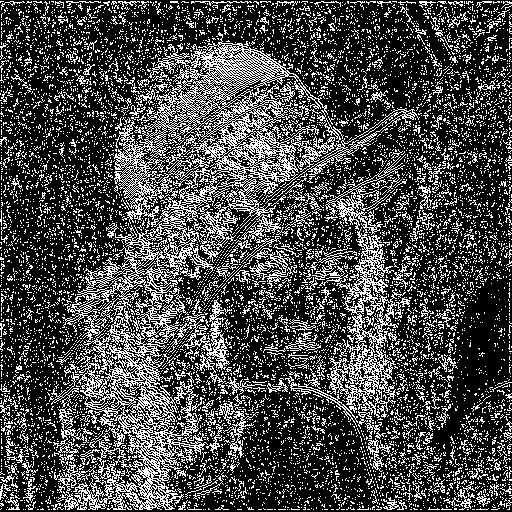
\includegraphics[width=8cm]{lena12.png}}
\caption{window size = $3$, $\sigma=0.5$,  threshold = $30$}
\label{lena12}
\end{figure}

\begin{figure}[H]
\centerline{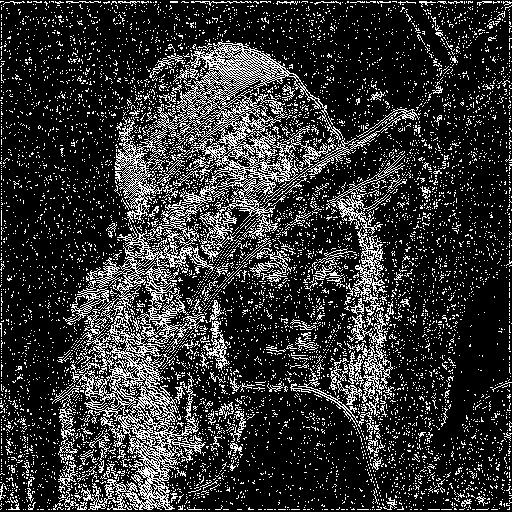
\includegraphics[width=8cm]{lena13.png}}
\caption{window size = $3$, $\sigma=0.5$,  threshold = $40$}
\label{lena13}
\end{figure}

\begin{figure}[H]
\centerline{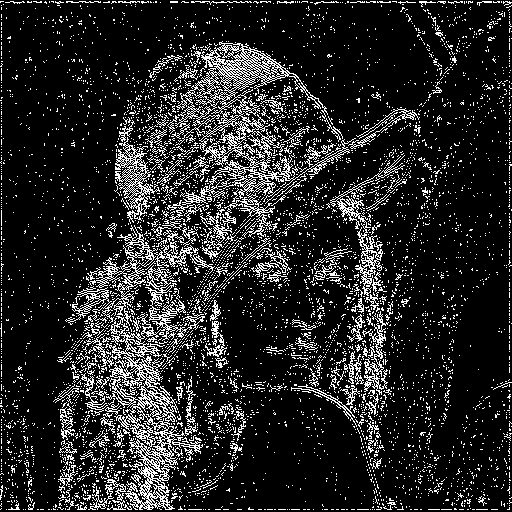
\includegraphics[width=8cm]{lena14.png}}
\caption{window size = $3$, $\sigma=0.5$,  threshold = $0$}
\label{lena14}
\end{figure}

\subsection{headCT}

原圖

\begin{figure}[H]
\centerline{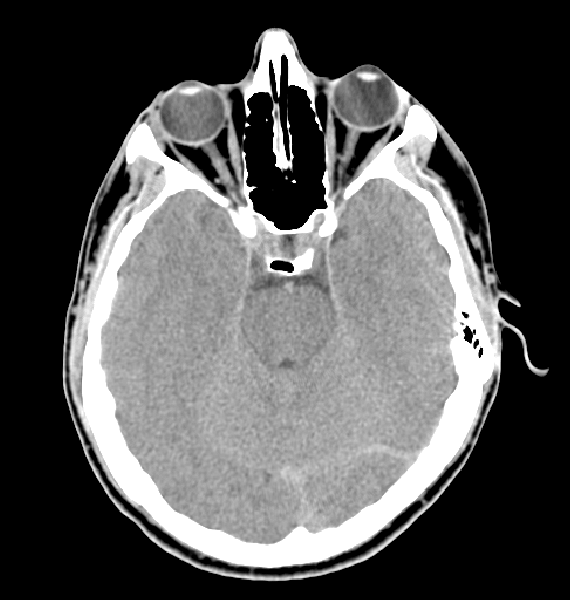
\includegraphics[width=8cm]{headCT.png}}
\caption{headCT}
\label{headCT}
\end{figure}

不同的 window size: 最明顯的差異在左上角, window size = $0.3$ 邊界是判斷最好的,$0.5$ 和 $0.7$ 時邊界消失。

\begin{figure}[H]
\centerline{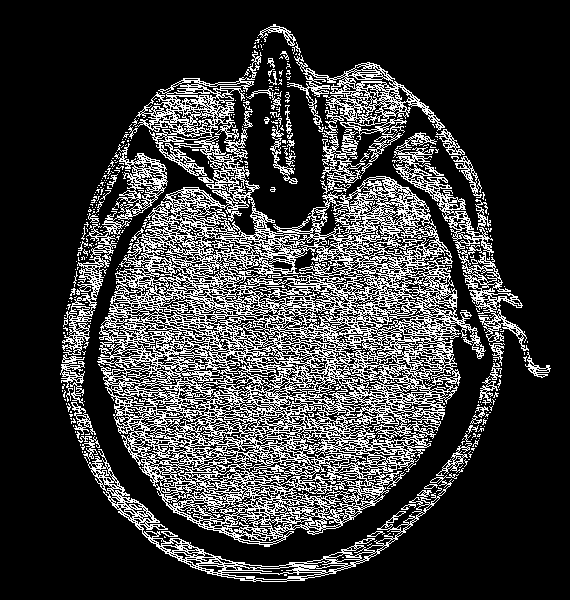
\includegraphics[width=8cm]{headCT01.png}}
\caption{window size = $3$, $\sigma=0.3$,  threshold = $30$}
\label{headCT01}
\end{figure}

\begin{figure}[H]
\centerline{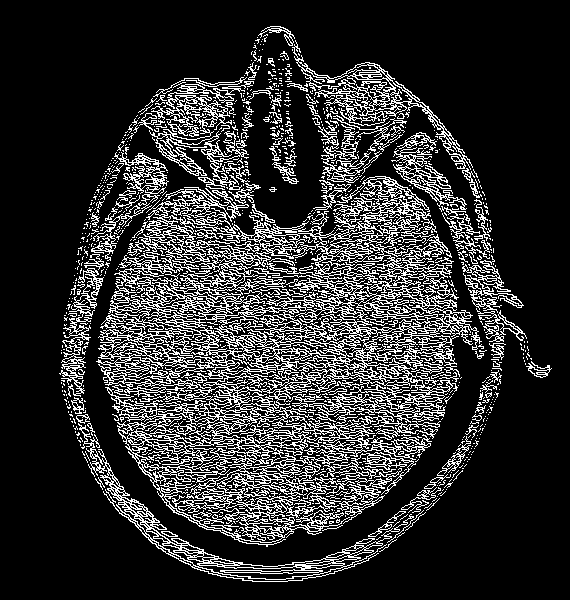
\includegraphics[width=8cm]{headCT02.png}}
\caption{window size = $5$, $\sigma=0.3$,  threshold = $30$}
\label{headCT02}
\end{figure}

\begin{figure}[H]
\centerline{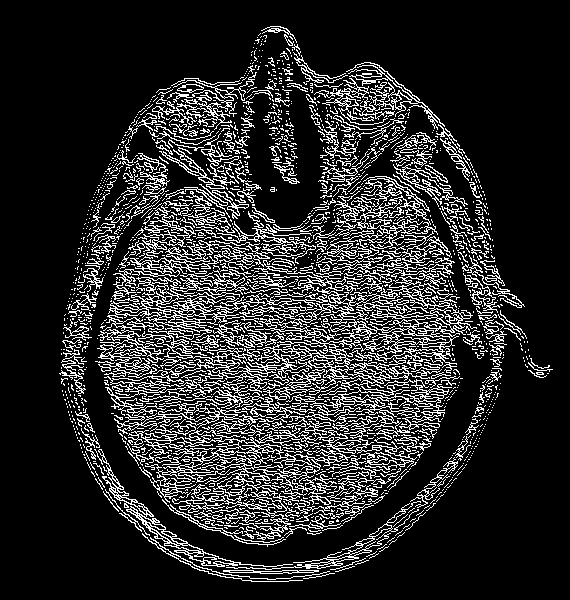
\includegraphics[width=8cm]{headCT03.png}}
\caption{window size = $7$, $\sigma=0.3$,  threshold = $30$}
\label{headCT03}
\end{figure}

不同的 $\sigma$: 當 $\sigma \geq 0.7$ 時,圓圈中間容易被判為邊界。


\begin{figure}[H]
\centerline{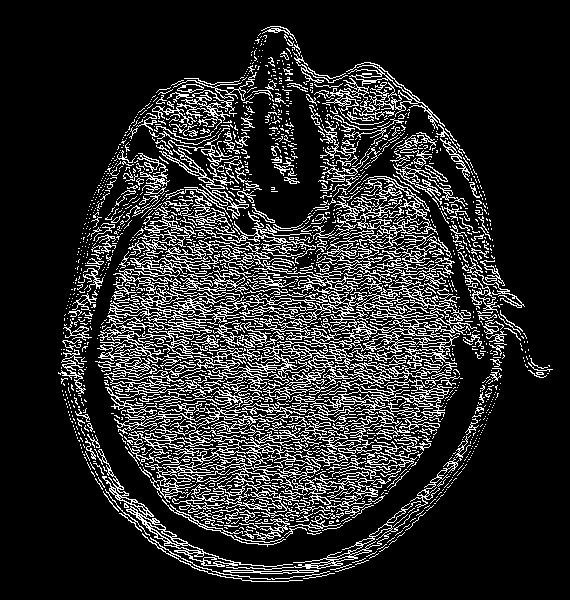
\includegraphics[width=8cm]{headCT04.png}}
\caption{window size = $7$, $\sigma=0.1$,  threshold = $40$}
\label{headCT04}
\end{figure}

\begin{figure}[H]
\centerline{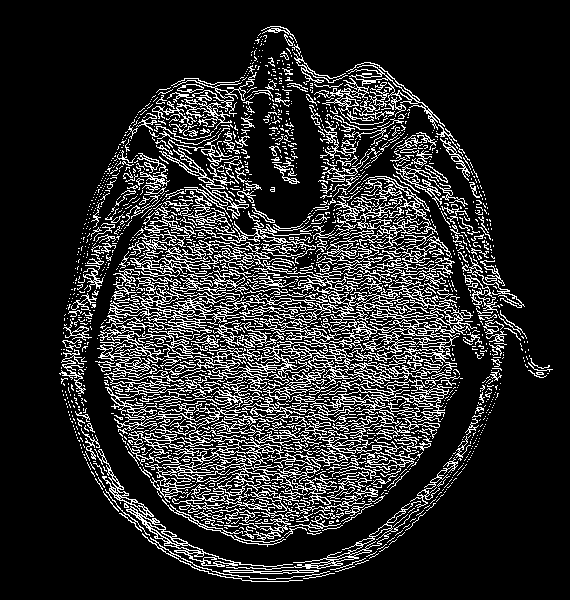
\includegraphics[width=8cm]{headCT05.png}}
\caption{window size = $7$, $\sigma=0.3$,  threshold = $40$}
\label{headCT05}
\end{figure}

\begin{figure}[H]
\centerline{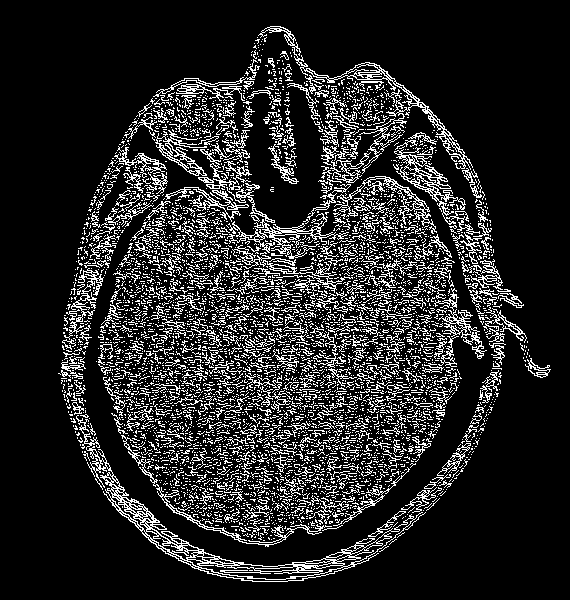
\includegraphics[width=8cm]{headCT06.png}}
\caption{window size = $7$, $\sigma=0.5$,  threshold = $40$}
\label{headCT06}
\end{figure}

\begin{figure}[H]
\centerline{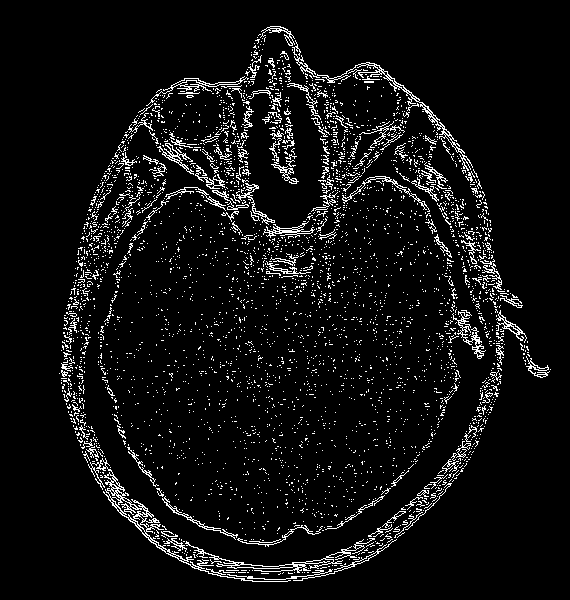
\includegraphics[width=8cm]{headCT07.png}}
\caption{window size = $7$, $\sigma=0.7$,  threshold = $40$}
\label{headCT07}
\end{figure}

\begin{figure}[H]
\centerline{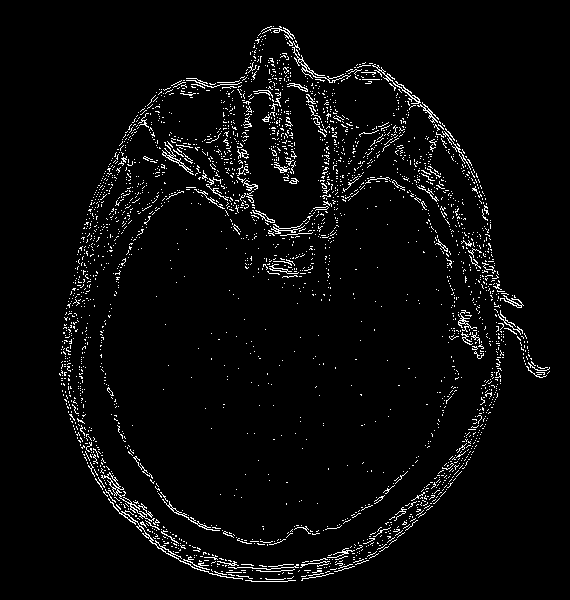
\includegraphics[width=8cm]{headCT08.png}}
\caption{window size = $7$, $\sigma=0.9$,  threshold = $40$}
\label{headCT08}
\end{figure}

不同的 thresold: thresold 越大,白色的區域密度降低。

\begin{figure}[H]
\centerline{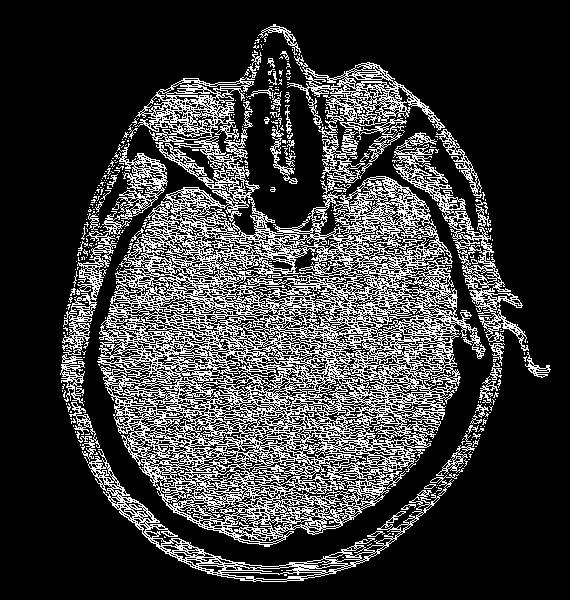
\includegraphics[width=8cm]{headCT09.png}}
\caption{window size = $3$, $\sigma=0.5$,  threshold = $0$}
\label{headCT9}
\end{figure}

\begin{figure}[H]
\centerline{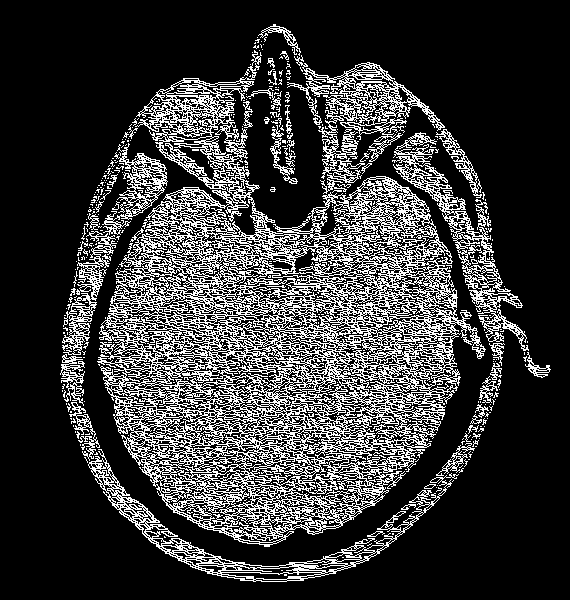
\includegraphics[width=8cm]{headCT10.png}}
\caption{window size = $3$, $\sigma=0.5$,  threshold = $10$}
\label{headCT10}
\end{figure}

\begin{figure}[H]
\centerline{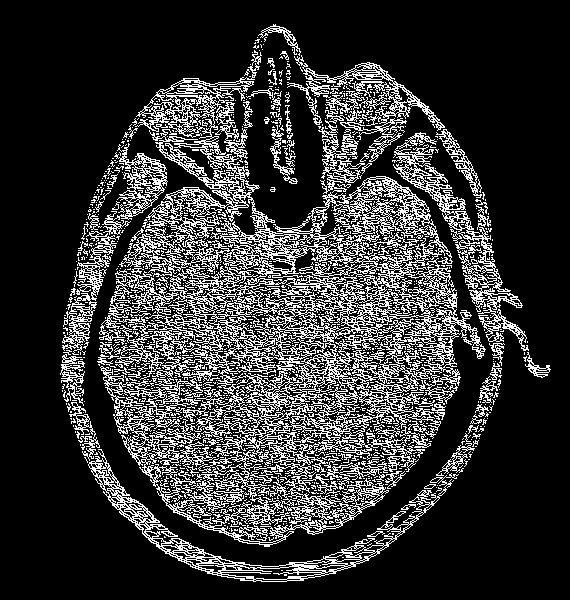
\includegraphics[width=8cm]{headCT11.png}}
\caption{window size = $3$, $\sigma=0.5$,  threshold = $20$}
\label{headCT11}
\end{figure}

\begin{figure}[H]
\centerline{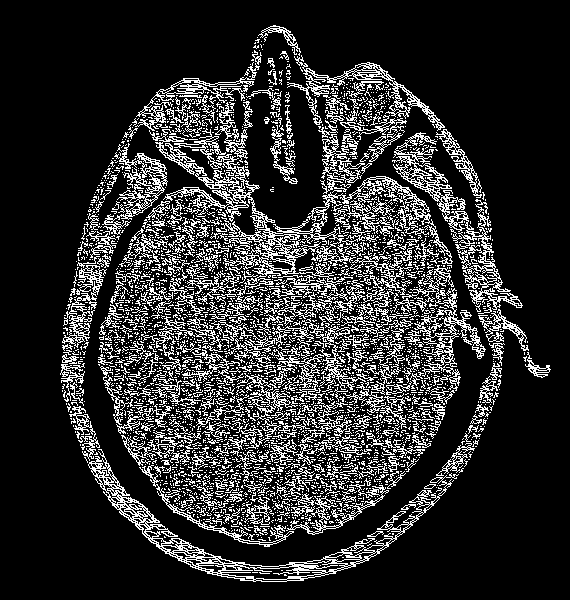
\includegraphics[width=8cm]{headCT12.png}}
\caption{window size = $3$, $\sigma=0.5$,  threshold = $30$}
\label{headCT12}
\end{figure}

\begin{figure}[H]
\centerline{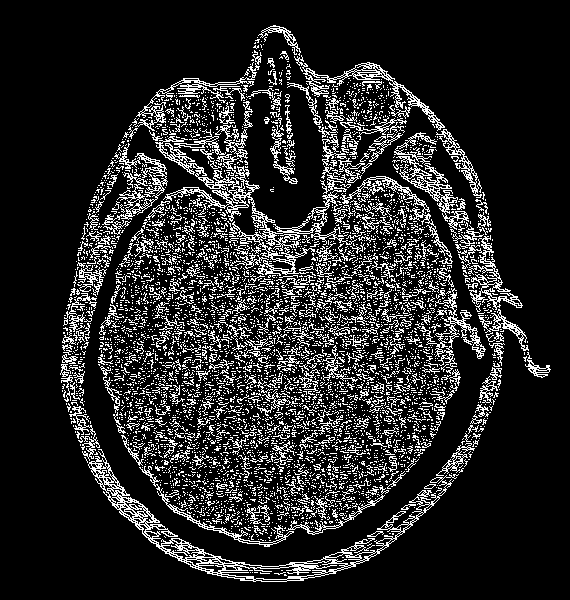
\includegraphics[width=8cm]{headCT13.png}}
\caption{window size = $3$, $\sigma=0.5$,  threshold = $40$}
\label{headCT13}
\end{figure}

\begin{figure}[H]
\centerline{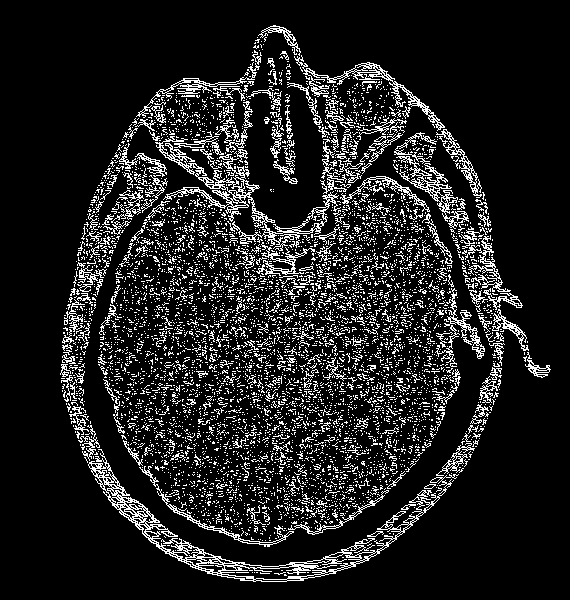
\includegraphics[width=8cm]{headCT14.png}}
\caption{window size = $3$, $\sigma=0.5$,  threshold = $0$}
\label{headCT14}
\end{figure}

\subsection{dentalXray}

原圖

\begin{figure}[H]
\centerline{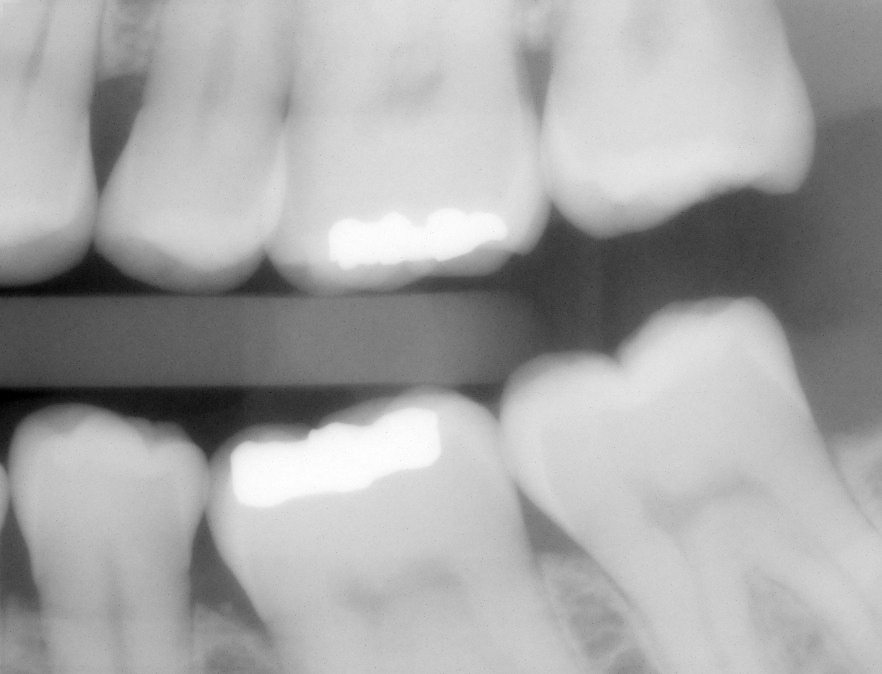
\includegraphics[width=8cm]{dentalXray.png}}
\caption{dentalXray}
\label{dentalXray}
\end{figure}

不同的 window size: window size$=7$ 時邊界的輪廓較清楚。

\begin{figure}[H]
\centerline{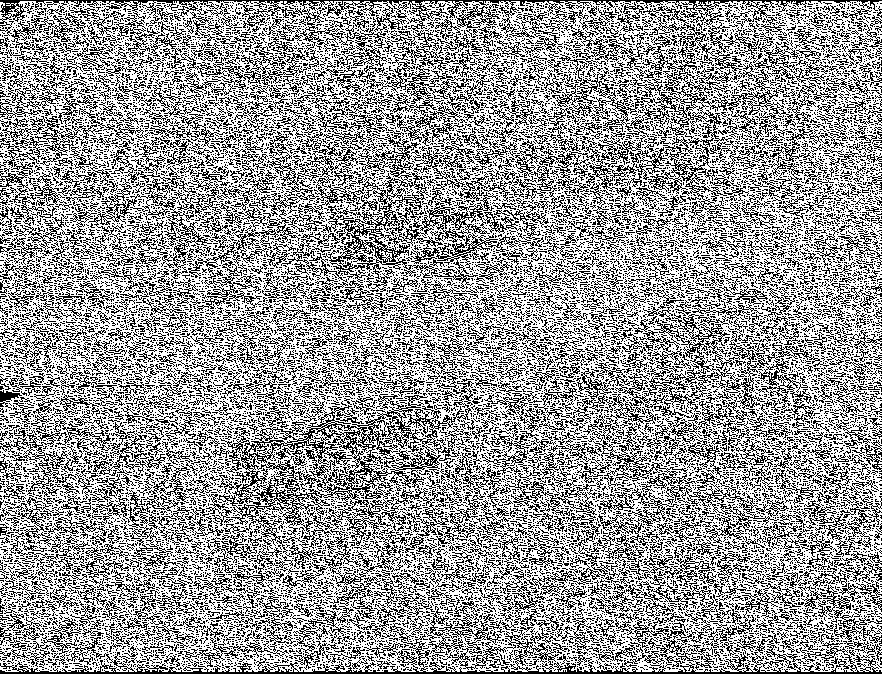
\includegraphics[width=8cm]{dentalXray01.png}}
\caption{window size = $3$, $\sigma=0.3$,  threshold = $30$}
\label{dentalXray01}
\end{figure}

\begin{figure}[H]
\centerline{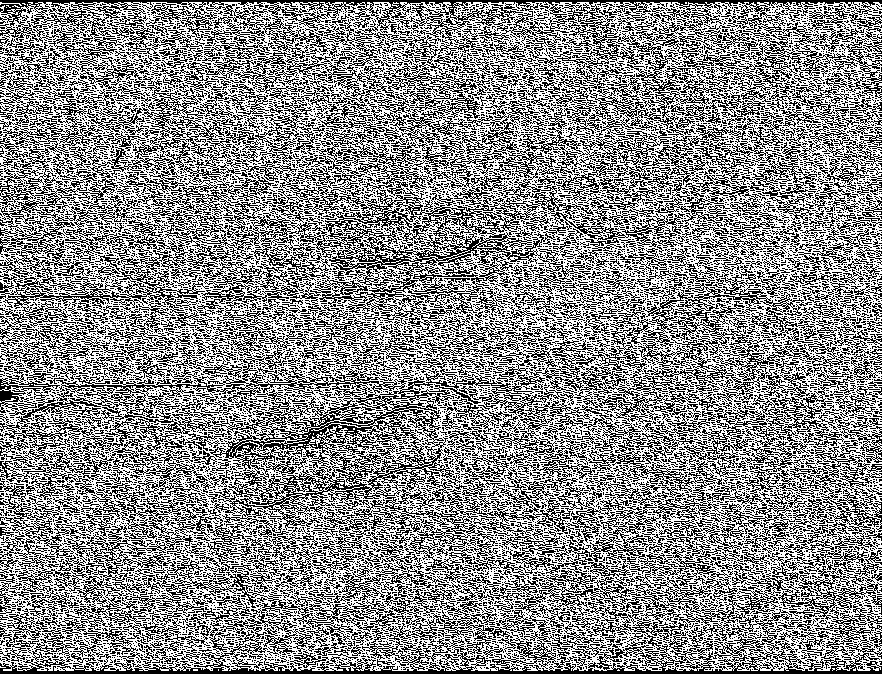
\includegraphics[width=8cm]{dentalXray02.png}}
\caption{window size = $5$, $\sigma=0.3$,  threshold = $30$}
\label{dentalXray02}
\end{figure}

\begin{figure}[H]
\centerline{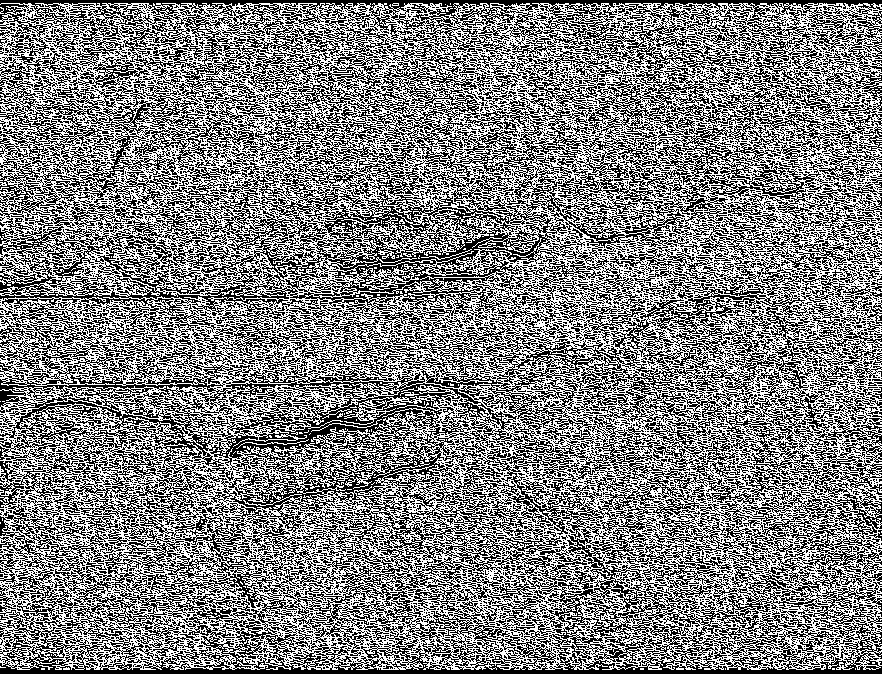
\includegraphics[width=8cm]{dentalXray03.png}}
\caption{window size = $7$, $\sigma=0.3$,  threshold = $30$}
\label{dentalXray03}
\end{figure}

不同的 $\sigma$: $\sigma=0.1,0.3$ 時,可以看到較正確的邊界,$\sigma\geq 0.5$ 時,大部分的點都被判斷為邊界,效果較差。


\begin{figure}[H]
\centerline{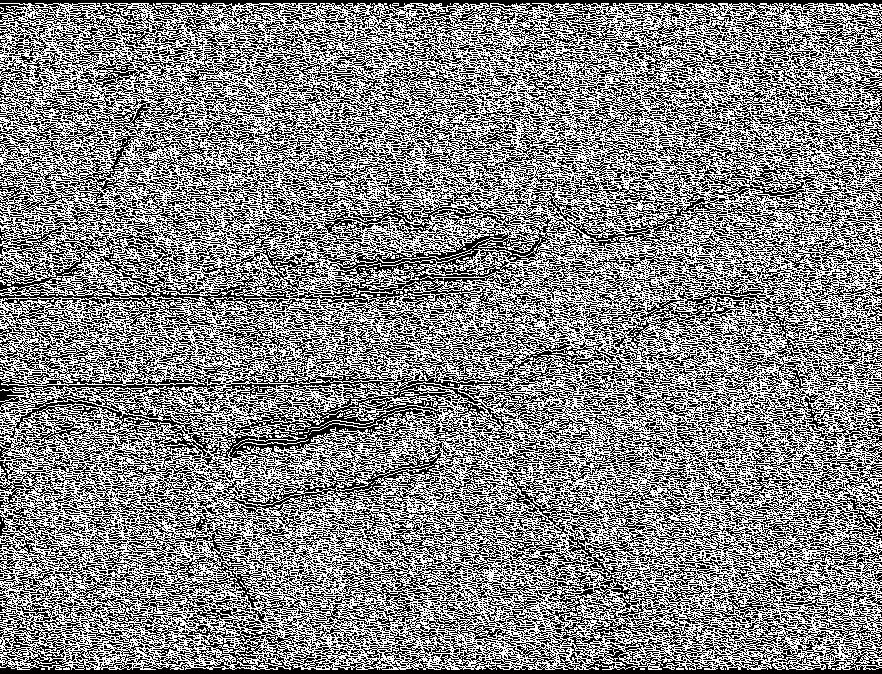
\includegraphics[width=8cm]{dentalXray04.png}}
\caption{window size = $7$, $\sigma=0.1$,  threshold = $40$}
\label{dentalXray04}
\end{figure}

\begin{figure}[H]
\centerline{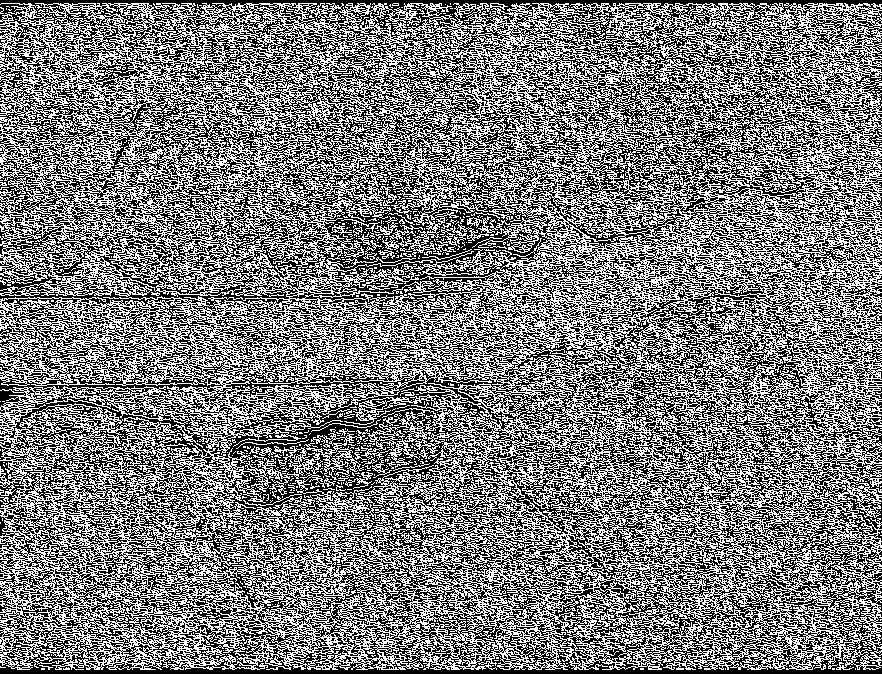
\includegraphics[width=8cm]{dentalXray05.png}}
\caption{window size = $7$, $\sigma=0.3$,  threshold = $40$}
\label{dentalXray05}
\end{figure}

\begin{figure}[H]
\centerline{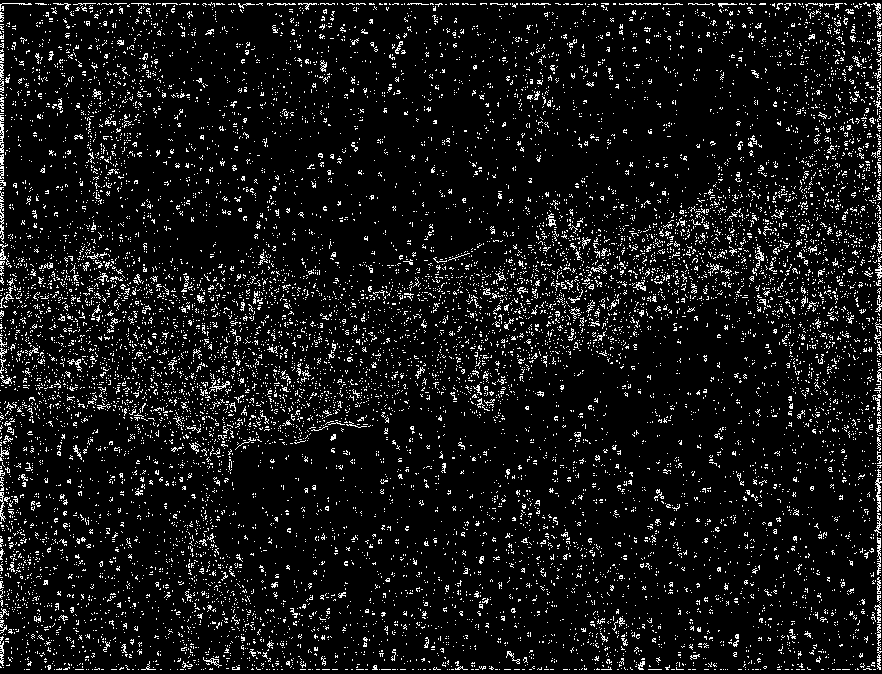
\includegraphics[width=8cm]{dentalXray06.png}}
\caption{window size = $7$, $\sigma=0.5$,  threshold = $40$}
\label{dentalXray06}
\end{figure}

\begin{figure}[H]
\centerline{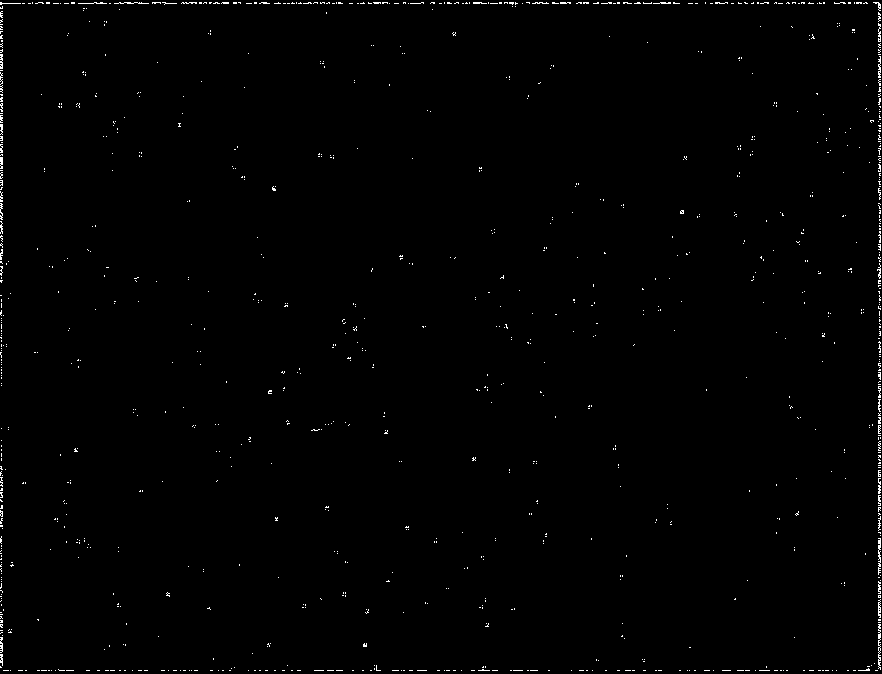
\includegraphics[width=8cm]{dentalXray07.png}}
\caption{window size = $7$, $\sigma=0.7$,  threshold = $40$}
\label{dentalXray07}
\end{figure}

\begin{figure}[H]
\centerline{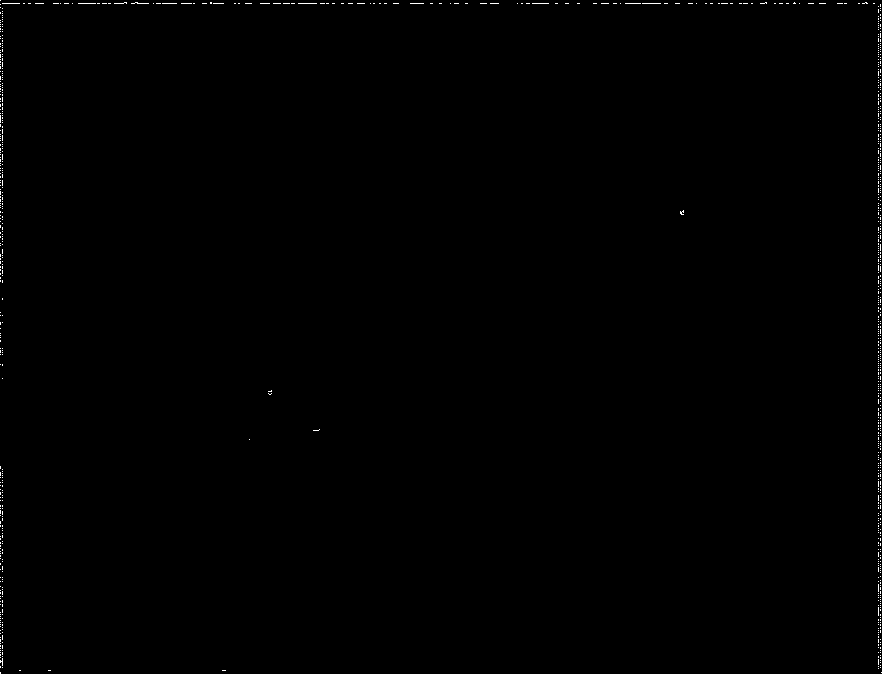
\includegraphics[width=8cm]{dentalXray08.png}}
\caption{window size = $7$, $\sigma=0.9$,  threshold = $40$}
\label{dentalXray08}
\end{figure}

不同的 thresold: 和上述兩張圖片類似,thresold 越大,白色的區域減少。

\begin{figure}[H]
\centerline{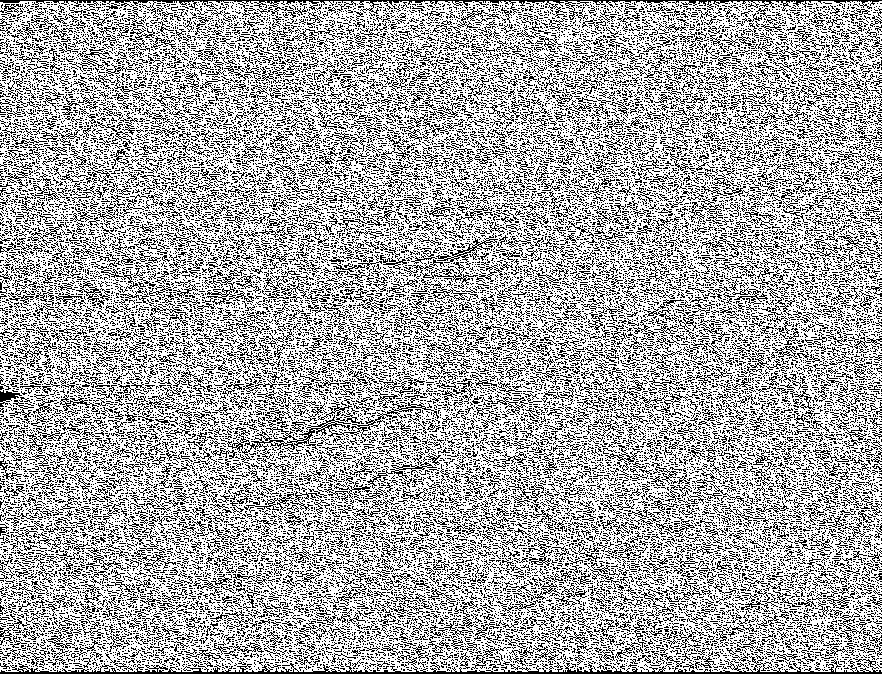
\includegraphics[width=8cm]{dentalXray09.png}}
\caption{window size = $3$, $\sigma=0.5$,  threshold = $0$}
\label{dentalXray9}
\end{figure}

\begin{figure}[H]
\centerline{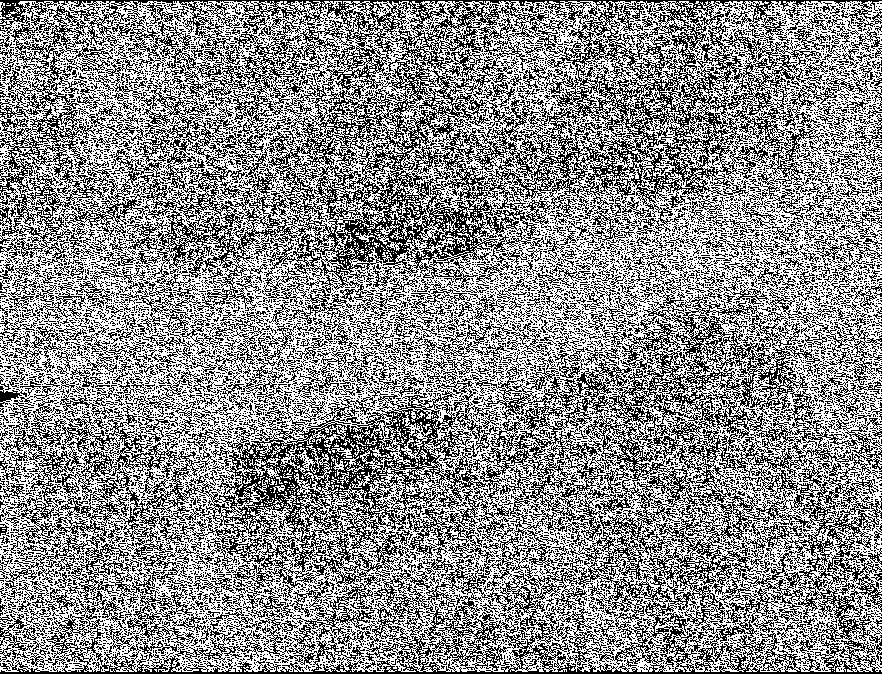
\includegraphics[width=8cm]{dentalXray10.png}}
\caption{window size = $3$, $\sigma=0.5$,  threshold = $10$}
\label{dentalXray10}
\end{figure}

\begin{figure}[H]
\centerline{
\includegraphics[width=8cm]{dentalXray11.png}}
\caption{window size = $3$, $\sigma=0.5$,  threshold = $20$}
\label{dentalXray11}
\end{figure}

\begin{figure}[H]
\centerline{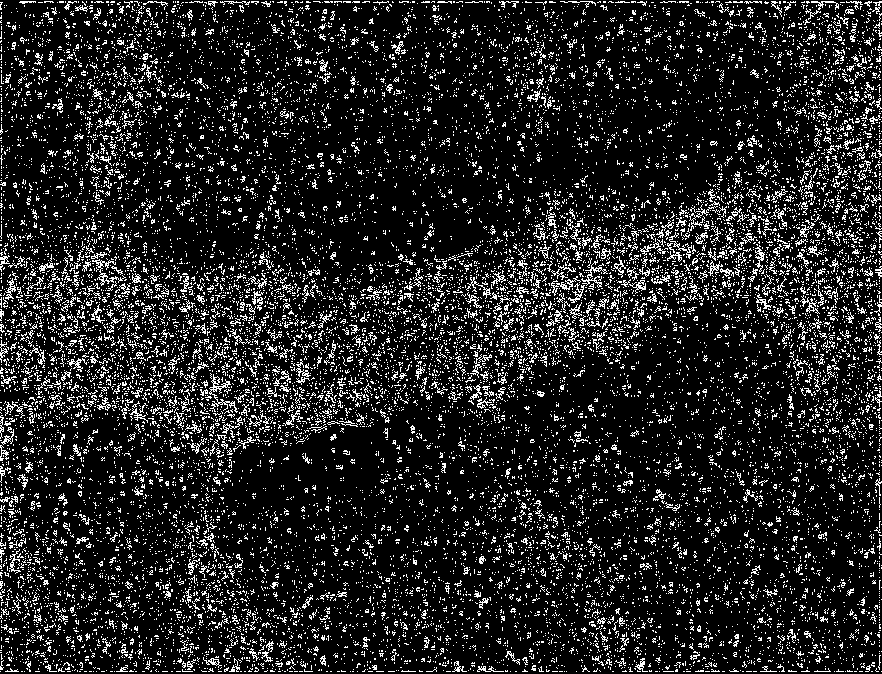
\includegraphics[width=8cm]{dentalXray12.png}}
\caption{window size = $3$, $\sigma=0.5$,  threshold = $30$}
\label{dentalXray12}
\end{figure}

\begin{figure}[H]
\centerline{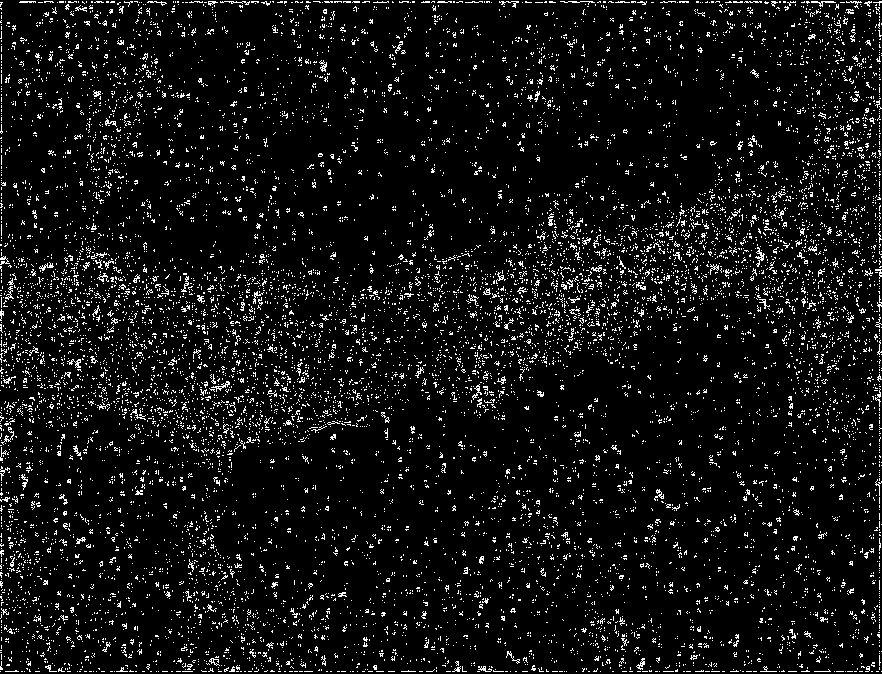
\includegraphics[width=8cm]{dentalXray13.png}}
\caption{window size = $3$, $\sigma=0.5$,  threshold = $40$}
\label{dentalXray13}
\end{figure}

\begin{figure}[H]
\centerline{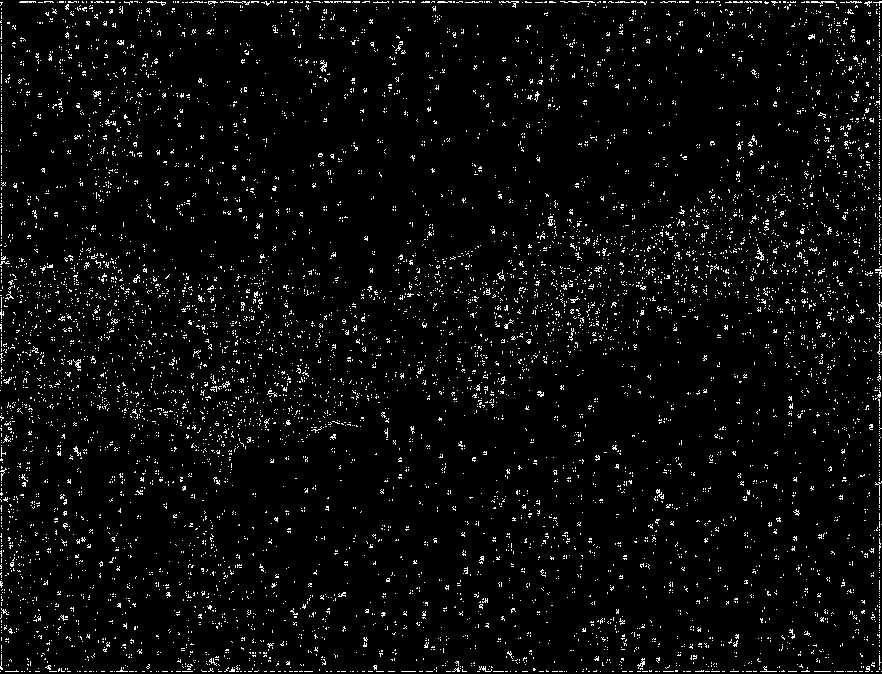
\includegraphics[width=8cm]{dentalXray14.png}}
\caption{window size = $3$, $\sigma=0.5$,  threshold = $0$}
\label{dentalXray14}
\end{figure}

\section{結語}
不同的 window size,對每張圖片的影響不同;不同的 $\sigma$ 和 threshold,會影響被判斷為邊界的比例多寡。不同的照片適合的參數不盡相同,需要多次實驗才能找出。

% % \begin{thebibliography}{00}
% % \end{thebibliography}

\vspace{12pt}

\end{document}
